\documentclass[journal]{IEEEtran}
\usepackage[a5paper, margin=10mm, onecolumn]{geometry}
\usepackage{lmodern} % Ensure lmodern is loaded for pdflatex
\usepackage{tfrupee} % Include tfrupee package

\setlength{\headheight}{1cm} % Set the height of the header box
\setlength{\headsep}{0mm}     % Set the distance between the header box and the top of the text

\usepackage{gvv-book}
\usepackage{gvv}
\usepackage{cite}
\usepackage{amsmath,amssymb,amsfonts,amsthm}
\usepackage{algorithmic}
\usepackage{graphicx}
\usepackage{textcomp}
\usepackage{xcolor}
\usepackage{txfonts}
\usepackage{listings}
\usepackage{enumitem}
\usepackage{mathtools}
\usepackage{gensymb}
\usepackage{comment}
\usepackage[breaklinks=true]{hyperref}
\usepackage{tkz-euclide} 
\usepackage{listings}                                      
\def\inputGnumericTable{}                                 
\usepackage[latin1]{inputenc}                                
\usepackage{color}                                            
\usepackage{array}                                            
\usepackage{longtable}
\usepackage{multicol}
\usepackage{calc}                                             
\usepackage{multirow}                                          
\usepackage{hhline}                                           
\usepackage{ifthen}                                           
\usepackage{lscape}

\begin{document}
	
\bibliographystyle{IEEEtran}
\vspace{3cm}

\title{11.16.3.8.3}
\author{EE24BTECH11047 - Niketh Prakash Achanta}
{\let\newpage\relax\maketitle}

\renewcommand{\thefigure}{\theenumi}
\renewcommand{\thetable}{\theenumi}
\setlength{\intextsep}{10pt} % Space between text and floats

\numberwithin{equation}{enumi}
\numberwithin{figure}{enumi}
\renewcommand{\thetable}{\theenumi}

\section{Problem Statement}
\textbf{Question}:\\
Three coins are tossed once. Find the probability of getting at least 2 heads.

\section{Solution}

\subsection{Random Variables}
Let $ X_1, X_2, X_3 $ be three independent random variables representing the outcomes of the three coin tosses:
\begin{align}
X_i =
\begin{cases}
1, & \text{if Head appears,} \\
0, & \text{if Tail appears.}
\end{cases}
\end{align}
Each $X_i$ follows a Bernoulli distribution with:
\begin{align}
P_{X}(1) = p = \frac{1}{2}, \quad P_{X}(0) = q = \frac{1}{2}.
\end{align}

\subsection{Probability Mass Function (PMF) Using Z-Transform}
The PMF of $X_i$ is:
\begin{align}
P_{X}(n) = p^{n} q^{1-n}.
\end{align}
The z-transform of this PMF is:
\begin{align}
P_{X_i}(z) = \mathbb{E}[z^{X_i}] = P_{X}(0) + P_{X}(1) z^{-1} = q + \frac{p}{z}.
\end{align}
For each $X_i$:
\begin{align}
P_{X_i}(z) = \frac{1}{2} + \frac{1}{2}z^{-1}.
\end{align}

\subsection{Distribution of $ Y = X_1 + X_2 + X_3 $}
Using the independence property, the z-transform of $Y$ is:
\begin{align}
P_Y(z) = P_{X_1}(z) \cdot P_{X_2}(z) \cdot P_{X_3}(z).
\end{align}
\begin{align}
P_Y(z) = \left(\frac{1}{2} + \frac{1}{2z}\right)^3.
\end{align}
Expanding, we get:
\begin{align}
P_Y(z) = \frac{1}{8} \left(1 + \frac{3}{z} + \frac{3}{z^2} + \frac{1}{z^3}\right).
\end{align}
Thus, the PMF of $Y$ is:
\begin{align}
P_{Y}(k) =
\begin{cases}
\frac{1}{8}, & k = 0, \\
\frac{3}{8}, & k = 1, \\
\frac{3}{8}, & k = 2, \\
\frac{1}{8}, & k = 3.
\end{cases}
\end{align}

We can also express this PMF in a summation notation:
\begin{align}
P_Y(k) = \sum_{k=0}^{3} P_Y(k) \quad \text{where} \quad P_Y(k) \in \left\{ \frac{1}{8}, \frac{3}{8} \right\}, \quad k = 0, 1, 2, 3.
\end{align}

\subsection{Cumulative Distribution Function (CDF)}
The CDF of $Y$ is:
\begin{align}
F_Y(k) =
\begin{cases}
0, & k < 0, \\
\frac{1}{8}, & 0 \leq k < 1, \\
\frac{4}{8}, & 1 \leq k < 2, \\
\frac{7}{8}, & 2 \leq k < 3, \\
1, & k \geq 3.
\end{cases}
\end{align}

\subsection{Probability of At Least Two Heads}
o get the probability of a particular event (Say 1 head), we take the coefficient of the corresponding power of z.
To find $ P(Y \geq 2) $, we use the coefficients of $z^{-2}$ and $z^{-3}$.\\
$\therefore$ Probability of At Least Two Heads = $\frac{1}{8} + \frac{3}{8} = \frac{1}{2}$
\section{Conclusion}
The probability that at least two of the three coin tosses result in heads is:
\begin{align}
P(Y \geq 2) = \frac{1}{2}.
\end{align}\\
We get the following plot.
\begin{figure}[!ht]
    \centering
    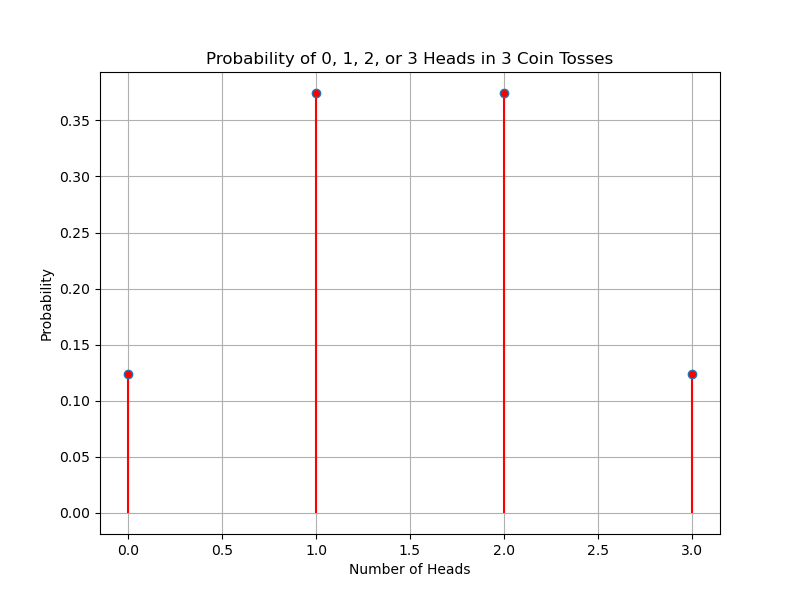
\includegraphics[width=\columnwidth]{/home/niketh/EE1003/3.8.3/figs/Figure_1.png}
    \caption{}
\end{figure}
\end{document}

